\let\negmedspace\undefined
\let\negthickspace\undefined

\documentclass[journal]{IEEEtran}
\usepackage[a5paper, margin=10mm, onecolumn]{geometry}
\usepackage{tfrupee}

\setlength{\headheight}{1cm}
\setlength{\headsep}{0mm}

\usepackage{gvv-book}
\usepackage{gvv}
\usepackage{cite}
\usepackage{amsmath,amssymb,amsfonts,amsthm}
\usepackage{algorithmic}
\usepackage{graphicx}
\usepackage{textcomp}
\usepackage{xcolor}
\usepackage{txfonts}
\usepackage{listings}
\usepackage{enumitem}
\usepackage{mathtools}
\usepackage{gensymb}
\usepackage{comment}
\usepackage[breaklinks=true]{hyperref}
\usepackage{tkz-euclide} 
\usepackage{listings}
\def\inputGnumericTable{}                                 
\usepackage[latin1]{inputenc}                                
\usepackage{color}                                            
\usepackage{array}                                            
\usepackage{longtable}                                       
\usepackage{calc}                                             
\usepackage{multirow}                                         
\usepackage{hhline}                                           
\usepackage{ifthen}                                           
\usepackage{lscape}
\begin{document}

\bibliographystyle{IEEEtran}
\vspace{3cm}

\title{7.4.17}
\author{EE25BTECH11010 - Arsh Dhoke}
{\let\newpage\relax\maketitle}

\renewcommand{\thefigure}{\theenumi}
\renewcommand{\thetable}{\theenumi}
\setlength{\intextsep}{10pt}
\numberwithin{equation}{enumi}
\numberwithin{figure}{enumi}
\renewcommand{\thetable}{\theenumi}

\parindent 0px
\textbf{Question}:\\
If the lines $2x + 3y + 1 = 0$ and $3x - y - 4 = 0$ lie along the diameter of a circle of circumference $10\pi$, then the equation of the circle is \hfill (2004)

\begin{enumerate}
\begin{multicols}{2}
\item $x^2 + y^2 + 2x - 2y - 23 = 0$
\item $x^2 + y^2 - 2x - 2y - 23 = 0$
\item $x^2 + y^2 + 2x + 2y - 23 = 0$
\item $x^2 + y^2 - 2x + 2y - 23 = 0$
\end{multicols}
\end{enumerate}
\solution \\ 
The equation of the circle is:($\vec{V}$ is an identity matrix of order = 2)
\begin{align}
\vec{x^T}\vec{V}\vec{x} + 2\vec{u^T}\vec{x} + f = 0 
\end{align}

\begin{align}
2x + 3y + 1 = 0 \\
3x - y - 4 = 0 
\end{align}
\begin{tabular}{|c|c|}
\hline
\textbf{Name} & \textbf{Value} \\ \hline
$\vec{A}$ & $\myvec{2 & 1 \\0 & 3}$ \\ \hline
\end{tabular}

\begin{align}
\myvec{2 & 3 \\ 3 & -1}\vec{x} = \myvec{-1 \\ 4} \\
\end{align}
In augmented form: 
\begin{align}
\augvec{2}{2}{2 & 3 & -1 \\ 3 & -1 & 4}
\end{align}

Performing row operations:
\begin{align}
&\augvec{2}{2}{2 & 3 & -1 \\ 3 & -1 & 4}
\xrightarrow[R_2 \to R_2 - \frac{3}{2}R_1]{}
\augvec{2}{2}{2 & 3 & -1 \\ 0 & -\frac{11}{2} & \frac{11}{2}} \\
&\xrightarrow[R_2 \to \frac{2}{-11}R_2]{}
\augvec{2}{2}{2 & 3 & -1 \\ 0 & 1 & -1} \\
&\xrightarrow[R_1 \to R_1 - 3R_2]{}
\augvec{2}{2}{2 & 0 & 2 \\ 0 & 1 & -1} \\
&\xrightarrow[R_1 \to \frac{1}{2}R_1]{}
\augvec{2}{2}{1 & 0 & 1 \\ 0 & 1 & -1}
\end{align}

\begin{align}
\vec{x} &= \myvec{1 \\ -1} \\
\text{Hence, the centre of the circle is } 
\vec{c} &= \myvec{1 \\ -1}
\end{align}

Given circumference $10\pi \Rightarrow r = 5 \Rightarrow r^2 = 25.$

\begin{align}
\vec{x}^{T}\vec{V}\vec{x} + 2\vec{u}^{T}\vec{x} + f &= 0 \\
\vec{V} &= \vec{I}, \quad \vec{c} = -\vec{u} \\
\Rightarrow \vec{u} &= -\myvec{1 \\ -1} = \myvec{-1 \\ 1} \\
f &= \vec{c}^{T}\vec{V}\vec{c} - r^2 = 2 - 25 = -23
\end{align}

Final equation of the circle:
\begin{align}
(\vec{x})^{T}\vec{I}\vec{x}+ 2\myvec{-1 & 1}\vec{x}- 23 &= 0 \\
(\vec{x})^{T}\vec{x}+ 2\myvec{-1 & 1}\vec{x}- 23 &= 0
\end{align}
Put $\vec{x}=\myvec{x \\ y}$, option d will be the answer.

\begin{figure}[ht!]
\centering
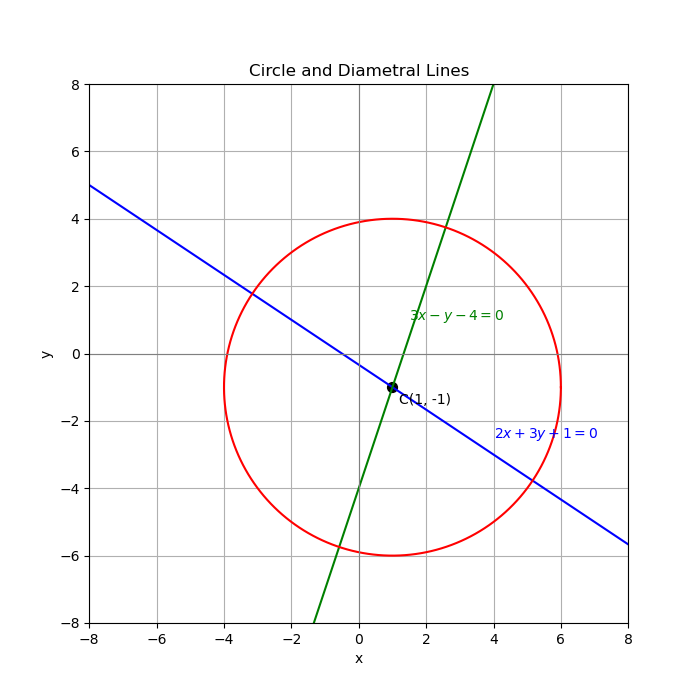
\includegraphics[height=0.6\textheight, keepaspectratio]{figs/circle.png}
\captionof{figure}{Graph}
\end{figure}

\end{document}